% !TEX root = ../main.tex
% 本文件由 build-tex.sh 从 13-DSP指南-第13章中译.md 生成，改内容请改 md 后重新生成

\chapter{连续信号处理}\label{ch-13}

连续信号处理(continuous signal processing)是与 DSP
平行的一个领域，大多数技术几乎完全相同。例如，DSP
和连续信号处理都建立在线性、分解、卷积和傅里叶分析之上。由于连续信号无法直接在数字计算机中表示，本章不会有计算机程序。连续信号处理以数学为基础：信号用方程表示，系统把一个方程变成另一个方程。正如数字计算机是
DSP
的主要工具，微积分是连续信号处理的主要工具。这些技术已经用了几百年，远在计算机出现之前。

\section{冲激函数}

和离散信号一样，连续信号也可以分解成一组经过缩放和平移的冲激函数(delta
function)。区别在于，连续冲激函数比离散的冲激函数复杂得多，也抽象得多。我们不去定义连续冲激函数''是什么''，而是用它具有的特性来定义它。

用一个思想实验来说明。设想一个由线性元件（比如电阻、电容和电感）组成的电子电路。输入端接一台信号发生器，能产生各种形状的短脉冲。电路的输出接示波器，显示电路对每个输入脉冲产生的波形。我们想回答的问题是：输出脉冲的形状和输入脉冲的特性有什么关系？为了简化研究，我们只用比输出短得多的输入脉冲。例如，如果系统的响应以毫秒计，我们可能只用几微秒长的输入脉冲。

做了大量测量之后，我们得出三个结论。第一，输入脉冲的形状不影响输出信号的形状。图
13-1
说明了这一点：各种形状的短输入脉冲产生的输出脉冲形状完全一样。第二，输出波形的形状完全由系统的特性决定，即电阻、电容和电感的取值和连接方式。第三，输出脉冲的幅度与输入脉冲的面积成正比。例如，输入为''1
伏持续 1 微秒''\,``10 伏持续 0.1 微秒''``1000 伏持续 1
纳秒''等时，输出的幅度都相同。这个关系也允许输入脉冲的面积为负。例如，设想一个
2 伏、持续 2 微秒的脉冲，紧接着一个 −1 伏、持续 4
微秒的脉冲。输入信号的总面积为零，于是输出什么也不做。

足够短、具备这三个性质的输入信号叫冲激(impulse)。换句话说，冲激就是除一个形状任意的短促尖峰外全为零的信号。例如，对微波发射机来说，冲激可能要短到皮秒量级，因为它的电子器件以纳秒为单位响应。相比之下，一次持续好几年的火山喷发，对需要上千年才发生的地质变化来说，完全可以算一个冲激。

数学家不喜欢被某个具体系统束缚，常用''冲激''一词指一个短到对任何可能的系统都算冲激的信号，也就是无穷窄的信号。连续冲激函数就是这种冲激的归一化版本。具体地说，连续冲激函数在数学上由三条理想化的特性定义：(1)
信号必须无穷短；(2) 脉冲必须出现在时间零点；(3) 脉冲的面积必须为一。

既然冲激函数被定义为无穷窄、面积固定，那么它的幅度就隐含为无穷大。别为此烦恼，这完全无关紧要。幅度是冲激''形状''的一部分，你永远不会遇到幅度起作用的问题，不管它是不是无穷大。冲激函数是一个数学构造，不是真实世界的信号。真实世界中充当冲激函数的信号，总是有有限的持续时间和幅度。

和离散情形一样，连续冲激函数用数学符号 δ( )
表示。同样，连续系统对冲激函数的输出叫冲激响应(impulse response)，常记作
h( )。注意，连续信号用圆括号 ( ) 表示，而离散信号用方括号 {[}
{]}。本书和 DSP
的其他文献都用这种记法，但它并不通用。在图中，冲激画成竖直的箭头（见图
13-1d），箭头的长度表示冲激的面积。

为了更好地理解真实世界中的冲激，在夜里看看天空中的一颗行星和一颗恒星，比如火星和天狼星。用肉眼看，两者的亮度和大小差不多。这种相似的原因并不明显，因为观看的几何条件相差悬殊。火星直径约
6000 千米，离地球约 6000 万千米。相比之下，天狼星大约大 300
倍，远一百多万倍。按这些尺寸，火星看起来应该比天狼星大三千多倍。它们怎么会看起来一样呢？

\begin{figure}[htbp]
\centering
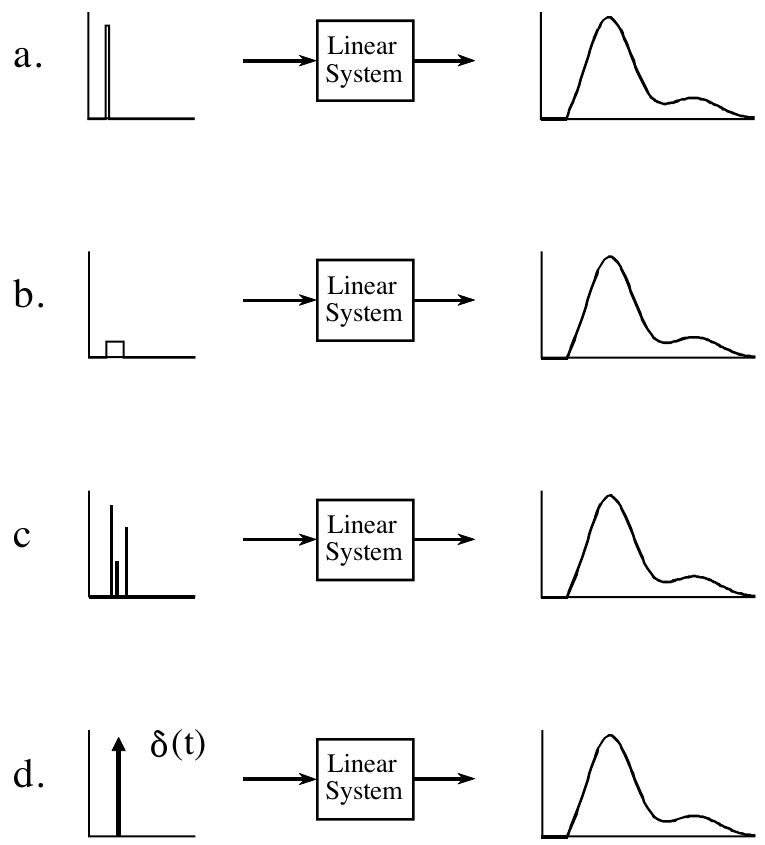
\includegraphics[width=0.637\linewidth,height=0.8\textheight,keepaspectratio]{assets/ch13/fig13-01.png}
\caption*{\textbf{图 13-1　连续冲激函数。}
如果线性系统的输入相对于它产生的输出很短，输出的形状就只取决于系统的特性，而与输入的形状无关。这样短的输入信号叫冲激。a、b、c
是对这个特定系统而言属于冲激的几种输入信号示例。冲激函数一词用来描述归一化的冲激，即出现在
t = 0、面积为一的冲激。(d) 给出了冲激函数的数学符号：一个竖直箭头和
δ(t)。 （Linear System = 线性系统。原书图注里 ``Figures a,b \& c'' 的 c
在图中缺了句点，无关紧要。）}
\end{figure}

它们看起来一样，是因为它们都小到对人类视觉系统来说算是冲激。我们感知到的形状是眼睛的冲激响应，而不是恒星或行星的真实图像。用一架小望远镜观察时这一点就很明显了：火星显出一个暗淡的圆盘，而天狼星仍然是一个明亮的冲激。这也是恒星会闪烁而行星不会的原因。恒星的像小到可以被大气中的颗粒或湍流短暂遮挡，而行星较大的像受到的影响要小得多。

\section{卷积}

和离散信号一样，连续信号的卷积(convolution)既可以从输入信号的角度看，也可以从输出信号的角度看。输入端视角最适合在概念上描述卷积怎样运作；输出端视角则描述了必须使用的数学。这些描述与第
6 章中离散信号的描述几乎完全一样。

图 13-2 展示了从输入端看卷积。输入信号 x(t) 通过一个以冲激响应 h(t)
刻画的系统，产生输出信号
y(t)。这可以写成熟悉的数学式：\(y(t) = x(t) * h(t)\)。输入信号被分成许多窄条，每一条都短到对系统来说算一个冲激。换句话说，输入信号被分解成无穷多个经过缩放和平移的冲激函数。每个冲激在输出信号中产生一个经过缩放和平移的冲激响应。最终的输出信号等于它们的综合效果，即所有单个响应之和。

\begin{figure}[htbp]
\centering
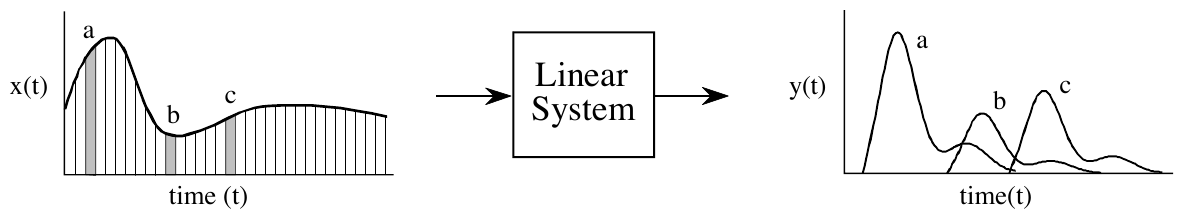
\includegraphics[width=0.988\linewidth,height=0.8\textheight,keepaspectratio]{assets/ch13/fig13-02.png}
\caption*{\textbf{图 13-2　从输入端看卷积。} 输入信号 x(t)
被分成许多窄段，每一段对系统来说都是一个冲激。输出信号 y(t)
是由此产生的、经过缩放和平移的各冲激响应之和。本图展示了输入信号中的三个点（a、b、c）怎样对输出信号作出贡献。
（Linear System = 线性系统，time (t) = 时间 (t)。）}
\end{figure}

要让这个方案行得通，窄条的宽度必须远小于系统响应的长度。当然，数学家会把它推到极致，让输入段无穷窄，把问题变成一个微积分问题。这样，输入端视角描述的就是输入信号中的一个点（或一个窄区域）怎样影响输出信号中较大的一段。

相比之下，输出端视角考察的是输出信号中的一个点怎样由输入信号的各个值决定。和离散信号一样，输出信号中的每个瞬时值都受输入信号中一段区间的影响，权重由左右翻转后的冲激响应给出。离散情形下，信号相乘后求和；连续情形下，信号相乘后积分。写成公式：

\textbf{公式 13-1}　卷积积分。这个公式定义了 \(y(t) = x(t) * h(t)\)
的含义。

\[y(t) = \int_{-\infty}^{+\infty} x(\tau)\, h(t-\tau)\, d\tau\]

这个公式叫卷积积分(convolution integral)，它是离散信号所用的卷积和（公式
6-1）的孪生兄弟。图 13-3
说明了怎样理解这个公式。目标是找到一个表达式，能算出输出信号在任意时刻 t
的值。第一步是更换用来遍历输入信号和冲激响应的自变量，即把 t 换成
τ（希腊字母 tau 的小写）。这样 x(t) 和 h(t) 分别变成 x(τ) 和
h(τ)。之所以要换变量名，是因为 t
已经用来表示正在计算的输出信号中的那个点了。下一步是把冲激响应左右翻转，变成
h(−τ)。再把翻转后的冲激响应平移到位置 t，表达式就变成
h(t−τ)。然后把输入信号与翻转并平移后的冲激响应相乘，对输入信号加权，即
x(τ)
h(t−τ)。最后，把这个加权后的输入信号从负无穷到正无穷积分，就得到输出信号的值，正如公式
13-1 所描述的。

如果你理解起来有困难，回头复习一下第 6 章中离散信号的同样概念。图 13-3
只不过是描述图 6-8
卷积机的另一种方式。唯一的区别是用积分代替了求和。把它当作你已知内容的扩展，而不是什么新东西。

\begin{figure}[htbp]
\centering
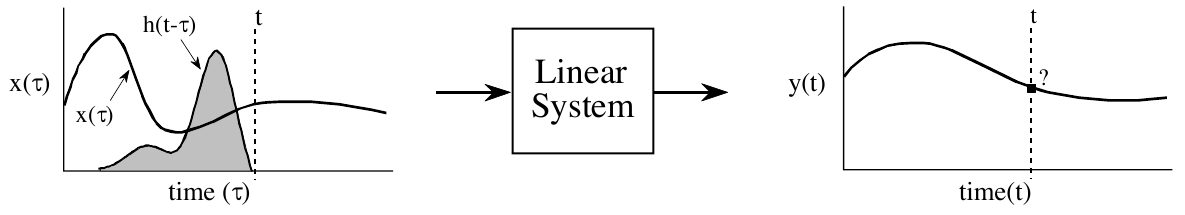
\includegraphics[width=0.988\linewidth,height=0.8\textheight,keepaspectratio]{assets/ch13/fig13-03.png}
\caption*{\textbf{图 13-3　从输出端看卷积。}
输出信号中的每个值都受输入信号中许多点的影响。本图中正在计算的是输出信号在时刻
t 的值。输入信号 x(τ) 被翻转并平移后的冲激响应 h(t−τ)
加权（相乘）。对加权后的输入信号积分，就得到输出点 y(t) 的值。 （Linear
System = 线性系统，time (τ) = 时间 (τ)；y(t) 图上的 ``?''
表示正在求的输出值。）}
\end{figure}

一个例子能说明连续卷积在实际问题中怎样使用、需要什么样的数学。图 13-4
是一个简单的连续线性系统：由一个电阻和一个电容组成的电子低通滤波器。如图所示，一个冲激进入这个系统后，输出会迅速跳到某个值，然后按指数衰减趋于零。换句话说，这个简单电子电路的冲激响应是一个单边指数(one-sided
exponential)。在数学上，这个系统的冲激响应分成两段，每段用一个方程表示：

\[h(t) = 0 \qquad t < 0\]

\[h(t) = \alpha e^{-\alpha t} \qquad t \ge 0\]

\begin{figure}[htbp]
\centering
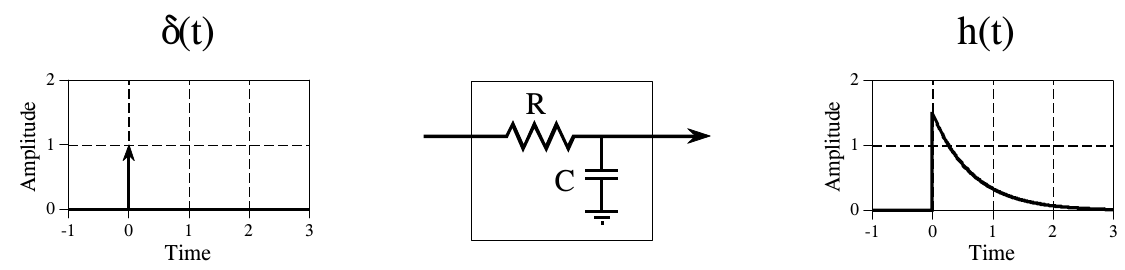
\includegraphics[width=0.938\linewidth,height=0.8\textheight,keepaspectratio]{assets/ch13/fig13-04.png}
\caption*{\textbf{图 13-4　连续线性系统的例子。}
这个电子电路是由一个电阻和一个电容组成的低通滤波器。该系统的冲激响应是一个单边指数。
（Amplitude = 幅度，Time = 时间；R = 电阻，C = 电容。）}
\end{figure}

其中 \(\alpha = 1/RC\)（R 以欧姆为单位，C 以法拉为单位，t
以秒为单位）。和离散情形一样，连续冲激响应包含了系统的全部信息，即它对一切可能信号的反应。把这个例子继续下去，图
13-5 展示了一个方波脉冲进入这个系统，用数学表示为：

\[x(t) = 1 \qquad 0 \le t \le 1\]

\[x(t) = 0 \qquad \text{其他}\]

\begin{figure}[htbp]
\centering
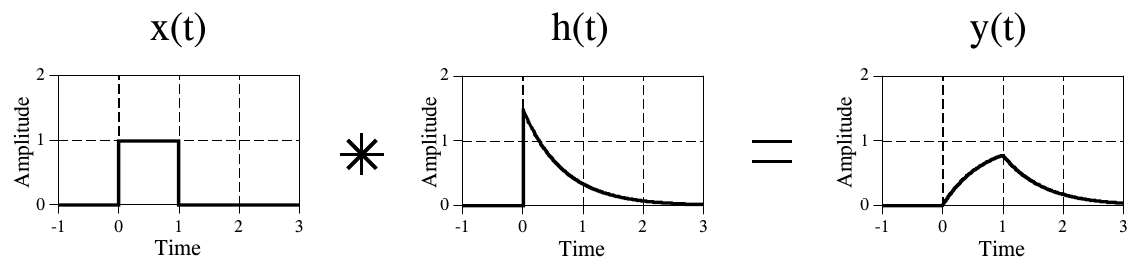
\includegraphics[width=0.946\linewidth,height=0.8\textheight,keepaspectratio]{assets/ch13/fig13-05.png}
\caption*{\textbf{图 13-5　连续卷积的例子。} 本图展示一个方波脉冲进入 RC
低通滤波器（图 13-4）。方波脉冲与系统的冲激响应卷积，得到输出。
（Amplitude = 幅度，Time = 时间。）}
\end{figure}

由于输入信号和冲激响应都已完全用数学表达式给出，输出信号 y(t)
就可以通过计算公式 13-1
的卷积积分求出。麻烦在于，两个信号都是分段定义的，而不是一个统一的数学表达式。这在连续信号处理中非常常见。通常必须画一张图，看清
t 取不同值时两个信号怎样相互滑过。在本例中，图 13-6a 表明，当 t
\textless{} 0 时两个信号完全不重叠。这意味着两个信号的乘积沿 τ
轴处处为零，得到的输出信号是：

\[y(t) = 0 \qquad t < 0\]

\begin{figure}[htbp]
\centering
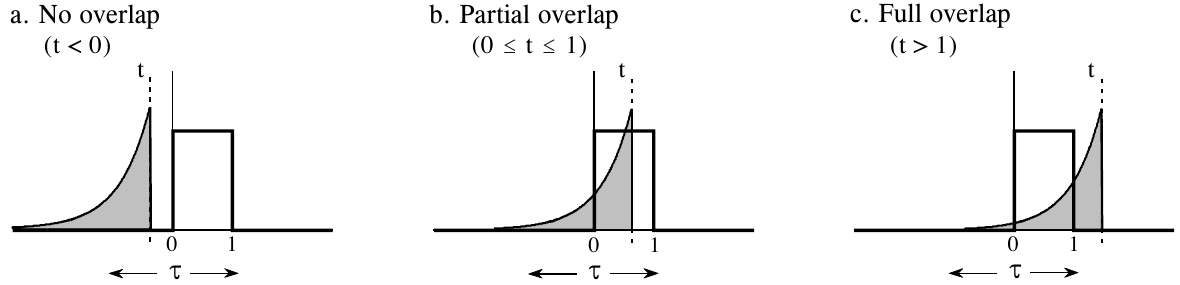
\includegraphics[width=0.983\linewidth,height=0.8\textheight,keepaspectratio]{assets/ch13/fig13-06.png}
\caption*{\textbf{图 13-6　分段计算卷积。}
由于许多连续信号是分段定义的，卷积计算也必须一段一段地做。本例中，输出信号的计算分成三段：输入信号与翻转平移后的冲激响应
(a) 不重叠，(b) 部分重叠，(c) 完全重叠。 （a. No overlap = 不重叠 (t
\textless{} 0)；b. Partial overlap = 部分重叠 (0 \dspsym{≤} t \dspsym{≤}
1)；c.~Full overlap = 完全重叠 (t \textgreater{} 1)。）}
\end{figure}

第二种情况见 (b)，此时 t 在 0 和 1 之间。两个信号部分重叠，它们的乘积在
τ = 0 到 τ = t
之间不为零。既然这是唯一的非零区域，积分只需在这一段上计算。这样得到 0
\dspsym{≤} t \dspsym{≤} 1 时的输出信号：

\[
\begin{aligned}
y(t) &= \int_{-\infty}^{\infty} x(\tau)\, h(t-\tau)\, d\tau && \text{（从公式 13-1 出发）}\\
y(t) &= \int_{0}^{t} 1\cdot \alpha e^{-\alpha(t-\tau)}\, d\tau && \text{（代入信号）}\\
y(t) &= e^{-\alpha t}\,\Big[e^{\alpha\tau}\Big]_{0}^{t} && \text{（计算积分）}\\
y(t) &= e^{-\alpha t}\,\big[e^{\alpha t} - 1\big] && \text{（化简）}\\
y(t) &= 1 - e^{-\alpha t} && 0 \le t \le 1
\end{aligned}
\]

\begin{enumerate}
\def\labelenumi{(\alph{enumi})}
\setcounter{enumi}{2}
\tightlist
\item
  给出了输出信号第三段（t \textgreater{} 1）的计算。这时重叠发生在 τ = 0
  到 τ = 1 之间，计算与第二段相同，只是积分上下限变了：
\end{enumerate}

\[
\begin{aligned}
y(t) &= \int_{0}^{1} 1\cdot \alpha e^{-\alpha(t-\tau)}\, d\tau && \text{（代入公式 13-1）}\\
y(t) &= e^{-\alpha t}\,\Big[e^{\alpha\tau}\Big]_{0}^{1} && \text{（计算积分）}\\
y(t) &= \big[e^{\alpha} - 1\big]\, e^{-\alpha t} && t > 1
\end{aligned}
\]

这三段的波形应该和你的电子学知识吻合：(1)
输入信号变为非零之前，输出信号必须为零，也就是说，第一段为 y(t) = 0，t
\textless{} 0。(2) 阶跃出现时，RC 电路按指数上升去追赶输入，方程为
\(y(t) = 1 - e^{-\alpha t}\)。(3)
输入回到零时，输出按指数衰减趋于零，方程为
\(y(t) = k e^{-\alpha t}\)（其中
\(k = e^{\alpha} - 1\)，即开始放电前一刻电容上的电压）。

更复杂的波形也可以用同样的方法处理，只是数学的复杂度会迅速变得难以驾驭。面对一个棘手的连续卷积问题时，你需要花相当多的时间评估解题策略。如果一上来就盲目地算积分，很可能最后得到一团数学乱麻。一个常用策略是把其中一个信号拆成几个更简单的相加分量，分别做卷积。利用线性原理，把得到的各个波形加起来，就是原问题的答案。

图 13-7
展示了另一种策略：以某种线性方式修改其中一个信号，做卷积，再撤销原来的修改。在这个例子里，修改是求导，撤销则是积分。单位幅度方波脉冲的导数是两个冲激：第一个面积为一，第二个面积为负一。要理解这一点，可以想想反过来对这两个冲激求积分的过程。积分经过第一个冲激时，迅速从零升到一，即一个阶跃函数。经过那个负冲激后，信号的积分又迅速从一回到零，方波脉冲就完整了。

求导之所以能简化这个问题，是因为当其中一个信号由冲激组成时，卷积很容易。x′(t)
中的两个冲激各自向输出信号的导数 y′(t)
贡献一个经过缩放和平移的冲激响应。也就是说，一眼就能看出：\(y'(t) = h(t) - h(t-1)\)。然后代入
h(t) 的确切方程，再对表达式积分，就得到输出信号 y(t)。

\begin{figure}[htbp]
\centering
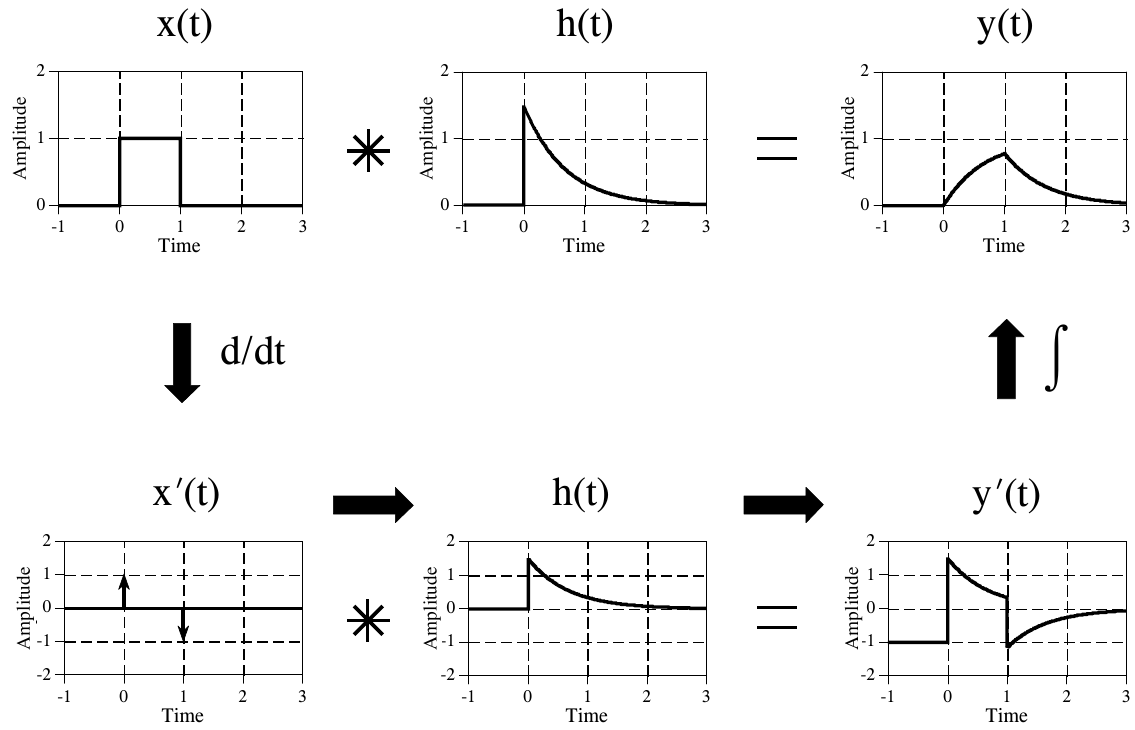
\includegraphics[width=0.946\linewidth,height=0.8\textheight,keepaspectratio]{assets/ch13/fig13-07.png}
\caption*{\textbf{图 13-7　一种卷积信号的策略。}
巧妙地运用线性系统的规则，常常能简化卷积问题。本例中，先对其中一个信号求导，从而简化两个信号的卷积。卷积完成后，再积分撤销求导。
（Amplitude = 幅度，Time = 时间；d/dt = 求导，\dspsym{∫} =
积分，\dspsym{∗} = 卷积。）}
\end{figure}

这个方法有一点小麻烦：求导时丢掉了输入信号的直流值(DC
value)。这可能导致算出的输出信号直流值有误。在数学上，这体现为积分时可以加上一个任意常数。没有系统的方法能识别这个误差，但通常可以通过检查问题来纠正。例如，图
13-7 的例子里就没有直流误差。之所以知道这一点，是因为 t
变得很大时，算出的输出信号有正确的直流值。如果某个问题中存在误差，就手动给输出信号加上一个合适的直流项来完成计算。

这个方法也适用于求几次导数后能化为冲激的信号。按这个领域的行话，这类信号叫分段多项式(piecewise
polynomial)。卷积之后，用多次积分撤销最初的多次求导。唯一的麻烦是，每一步都要找到正确的积分常数，把丢掉的直流值补回来。

在动手解一个困难的连续卷积问题之前，还有一种方法值得考虑。问问自己：输出信号真的需要一个数学表达式吗？还是有一张波形图就够了？如果一张图就够了，你也许最好用离散技术来处理这个问题，也就是用采样来近似连续信号，再用计算机程序直接做卷积。这样做虽然在数学上不那么纯粹，却可能容易得多。

\section{傅里叶变换}

连续信号的傅里叶变换分成两类：一类针对周期信号，一类针对非周期信号。周期信号使用的傅里叶变换版本叫傅里叶级数(Fourier
Series)，下一节讨论。用于非周期信号的就简单地叫傅里叶变换(Fourier
Transform)。和前几章讲离散信号时一样，本章只用实数数学来描述这些傅里叶技术。更强大的复数数学留到第
31 章。

图 13-8
是一个连续非周期信号及其频谱的例子。时域信号从负无穷延伸到正无穷，而频域的各个信号从零延伸到正无穷。这里的频谱用直角坐标形式（实部和虚部）表示；不过对连续信号也会用极坐标形式（幅度和相位）。和离散情形一样，合成方程(synthesis
equation)给出了用频域数据构造时域信号的配方。数学形式为：

\textbf{公式 13-2}　傅里叶变换合成方程。式中 x(t) 是被合成的时域信号，Re
X(ω) 和 Im X(ω) 分别是频谱的实部和虚部。

\[x(t) = \frac{1}{\pi}\int_{0}^{+\infty} \Big[\operatorname{Re}X(\omega)\cos(\omega t) - \operatorname{Im}X(\omega)\sin(\omega t)\Big]\, d\omega\]

用文字说，时域信号由无穷多个经过缩放的正弦和余弦波相加（借助积分）而成。频域的实部是余弦波的缩放系数，虚部是正弦波的缩放系数。和离散信号一样，合成方程通常写成带负号的正弦波。虽然这个负号在这里的讨论中没有意义，但它是让记法与第
31
章介绍的复数数学相容所必需的。要记住的关键一点是：有的作者在方程里加这个负号，有的不加。

\begin{quote}
\textbf{译注：} 原文此处写''第 29 章介绍的复数数学''，与本段前文''留到第
31 章''矛盾。本书讲复数 DFT 的是第 31 章，第 29 章是《DSP
上手实践》，这里按第 31 章译。
\end{quote}

还要注意，频率用符号 ω（希腊字母 omega
的小写）表示。你可能还记得，这种记法叫自然频率(natural
frequency)，单位是弧度每秒。也就是说，\(\omega = 2\pi f\)，其中 f
是以周每秒（赫兹）为单位的频率。用解方程的方式做信号处理的数学家和其他人偏爱自然频率记法，因为通常要写的符号更少。

\begin{figure}[htbp]
\centering
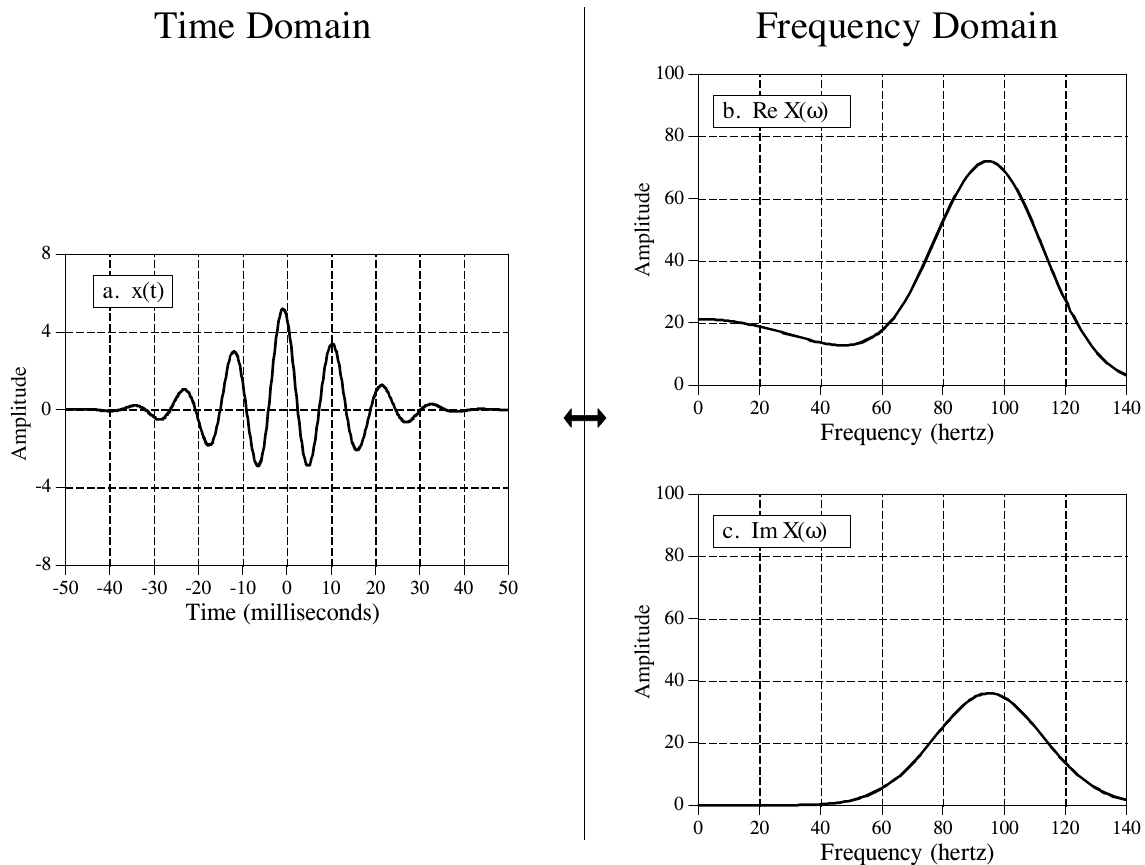
\includegraphics[width=0.954\linewidth,height=0.8\textheight,keepaspectratio]{assets/ch13/fig13-08.png}
\caption*{\textbf{图 13-8　傅里叶变换的例子。} 时域信号 x(t)
从负无穷延伸到正无穷。频域由实部 Re X(ω) 和虚部 Im X(ω)
组成，各自从零延伸到正无穷。本图的频率轴以周每秒（赫兹）标注。要换算成自然频率，把频率轴上的数乘以
2π。 （Time Domain = 时域，Frequency Domain = 频域；Amplitude =
幅度，Time (milliseconds) = 时间（毫秒），Frequency (hertz) =
频率（赫兹）。）}
\end{figure}

连续信号的分析方程(analysis
equation)沿用离散情形的思路：与正弦和余弦波做相关。方程为：

\textbf{公式 13-3}　傅里叶变换分析方程。式中 Re X(ω) 和 Im X(ω)
分别是频谱的实部和虚部，x(t) 是被分析的时域信号。

\[\operatorname{Re}X(\omega) = \int_{-\infty}^{+\infty} x(t)\cos(\omega t)\, dt\]

\[\operatorname{Im}X(\omega) = -\int_{-\infty}^{+\infty} x(t)\sin(\omega t)\, dt\]

作为使用分析方程的一个例子，我们来求 RC 低通滤波器的频率响应(frequency
response)。做法是对它的冲激响应做傅里叶变换。冲激响应前面已在图 13-4
中给出，描述为：

\[h(t) = 0 \qquad t < 0\]

\[h(t) = \alpha e^{-\alpha t} \qquad t \ge 0\]

把冲激响应代入分析方程，就能求出频率响应。先算实部：

\[
\begin{aligned}
\operatorname{Re}H(\omega) &= \int_{-\infty}^{+\infty} h(t)\cos(\omega t)\, dt && \text{（从公式 13-3 出发）}\\
\operatorname{Re}H(\omega) &= \int_{0}^{+\infty} \alpha e^{-\alpha t}\cos(\omega t)\, dt && \text{（代入信号）}\\
\operatorname{Re}H(\omega) &= \frac{\alpha e^{-\alpha t}}{\alpha^2+\omega^2}\Big[-\alpha\cos(\omega t) + \omega\sin(\omega t)\Big]_{0}^{+\infty} && \text{（计算）}\\
\operatorname{Re}H(\omega) &= \frac{\alpha^2}{\alpha^2+\omega^2}
\end{aligned}
\]

用同样的方法，算出频率响应的虚部为：

\[\operatorname{Im}H(\omega) = \frac{-\omega\alpha}{\alpha^2+\omega^2}\]

和离散信号一样，频域的直角坐标表示非常适合数学推导，却不便于人理解。把它换成极坐标就能解决这个问题，用标准关系式：\(\operatorname{Mag}H(\omega) = \big[\operatorname{Re}H(\omega)^2 + \operatorname{Im}H(\omega)^2\big]^{1/2}\)，以及
\(\operatorname{Phase}H(\omega) = \arctan\big[\operatorname{Im}H(\omega)/\operatorname{Re}H(\omega)\big]\)。

\begin{quote}
\textbf{译注：} 原文相位公式写成 arctan{[}Re H(ω) / Im
H(ω){]}，分子分母颠倒了。相位应为虚部除以实部（见第 8 章公式
8-6），下面的结果 arctan(−ω/α) 也正是按 Im/Re 算出的。
\end{quote}

经过代数运算，就得到 RC
低通滤波器以幅度和相位（即极坐标形式）表示的频率响应：

\[\operatorname{Mag}H(\omega) = \frac{\alpha}{\big[\alpha^2+\omega^2\big]^{1/2}}\]

\[\operatorname{Phase}H(\omega) = \arctan\left[-\frac{\omega}{\alpha}\right]\]

图 13-9 画出了截止频率为 1000 赫兹（即
\(\alpha = 2\pi\cdot 1000\)）时的这些曲线。

\begin{figure}[htbp]
\centering
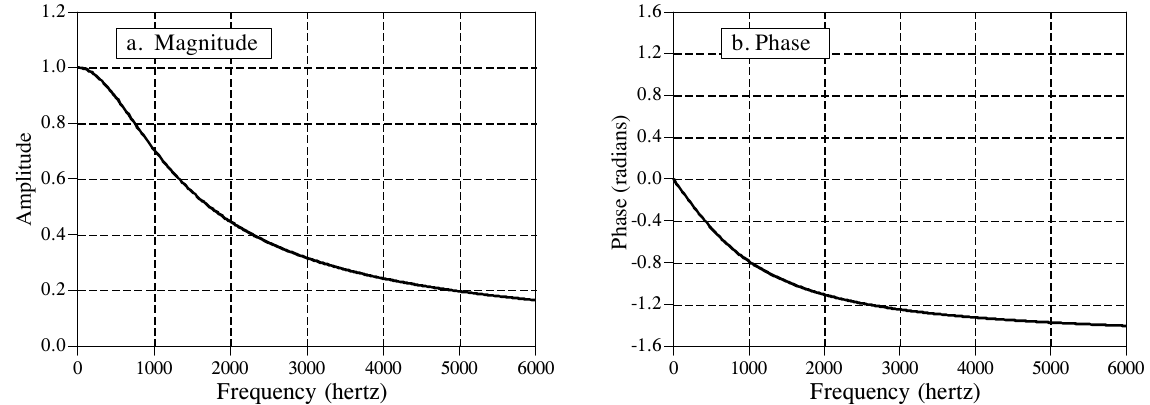
\includegraphics[width=0.958\linewidth,height=0.8\textheight,keepaspectratio]{assets/ch13/fig13-09.png}
\caption*{\textbf{图 13-9　RC 低通滤波器的频率响应。}
这些曲线是先对冲激响应做傅里叶变换，再换算成极坐标形式得到的。 （a.
Magnitude = 幅度；b. Phase = 相位。Amplitude = 幅度，Phase (radians) =
相位（弧度），Frequency (hertz) = 频率（赫兹）。）}
\end{figure}

\section{傅里叶级数}

这就讲到傅里叶变换家族的最后一位成员：傅里叶级数。傅里叶级数所用的时域信号是周期的、连续的。图
13-10 给出了几个从负无穷到正无穷不断重复的连续波形的例子。第 11
章讲过，周期信号的频谱由谐波(harmonic)组成。例如，如果时域以 1000
赫兹重复（周期 1 毫秒），频谱就会有 1000 赫兹的一次谐波、2000
赫兹的二次谐波、3000
赫兹的三次谐波，依此类推。一次谐波，即时域重复的频率，也叫基频(fundamental
frequency)。这意味着频谱可以用两种方式看待：(1)
频谱是连续的，但除谐波以外的所有频率上都为零；(2)
频谱是离散的，只在谐波频率上有定义。换句话说，谐波之间的频率可以看作取值为零，也可以看作根本不存在。重要的是，它们对形成时域信号没有贡献。

傅里叶级数合成方程把频率为 f、2f、3f、4f
等的经过缩放的余弦和正弦波加起来，构造出一个基频为 f
的连续周期信号。余弦波的幅度存放在变量 a₁、a₂、a₃、a₄
等中，正弦波的幅度存放在 b₁、b₂、b₃、b₄
等中。换句话说，``a''系数和''b''系数分别是频谱的实部和虚部。此外，系数
a₀
用来存放时域波形的直流值。它可以看作频率为零的余弦波（一个常数）的幅度。有时
a₀ 和其他''a''系数归在一起，但它常被单独处理，因为它需要特殊的计算。没有
b₀ 系数，因为频率为零的正弦波恒等于零，毫无用处。合成方程写作：

\textbf{公式 13-4}　傅里叶级数合成方程。任何周期信号 x(t)
都能由频率为基频 f 整数倍的正弦和余弦波重建出来。a\textsubscript{n} 和
b\textsubscript{n} 系数分别存放余弦波和正弦波的幅度。

\[x(t) = a_0 + \sum_{n=1}^{\infty} a_n\cos(2\pi f t n) - \sum_{n=1}^{\infty} b_n\sin(2\pi f t n)\]

傅里叶级数相应的分析方程，通常用波形的周期 T 而不是基频 f 来写（其中 f =
1/T）。由于时域信号是周期的，与正弦和余弦波的相关只需在一个周期上计算，即
−T/2 到 T/2、0 到 T、−T 到 0
等。选不同的积分限会让数学推导不同，但最终答案总是一样的。傅里叶级数分析方程为：

\textbf{公式 13-5}　傅里叶级数分析方程。式中 x(t) 是被分解的时域信号，a₀
是直流分量，a\textsubscript{n} 和 b\textsubscript{n}
分别存放余弦波和正弦波的幅度，T 是信号的周期，即基频的倒数。

\[a_0 = \frac{1}{T}\int_{-T/2}^{T/2} x(t)\, dt\]

\[a_n = \frac{2}{T}\int_{-T/2}^{T/2} x(t)\cos\!\left(\frac{2\pi t n}{T}\right) dt\]

\[b_n = \frac{-2}{T}\int_{-T/2}^{T/2} x(t)\sin\!\left(\frac{2\pi t n}{T}\right) dt\]

\begin{figure}[htbp]
\centering
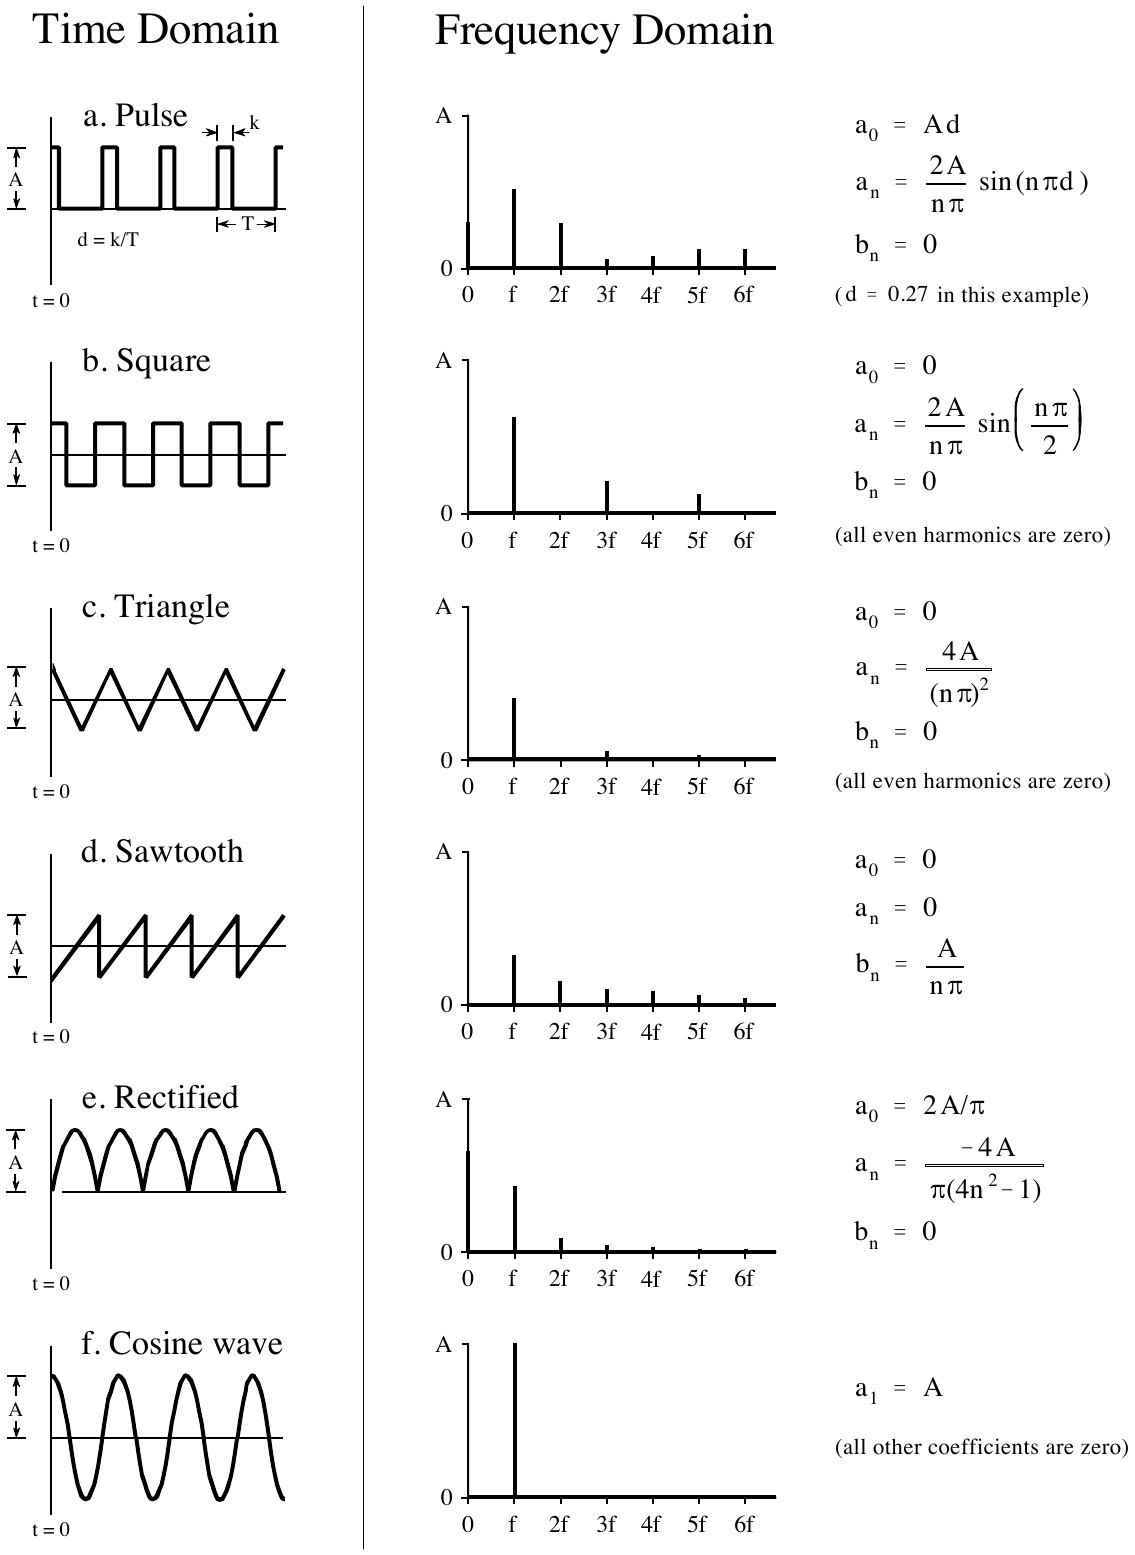
\includegraphics[width=0.946\linewidth,height=0.8\textheight,keepaspectratio]{assets/ch13/fig13-10.png}
\caption*{\textbf{图 13-10　傅里叶级数的例子。}
图中给出六种常见的时域波形，以及计算它们''a''\,``b''系数的公式。 （Time
Domain = 时域，Frequency Domain = 频域。六种波形依次为：a. Pulse =
脉冲（d = 0.27 in this example = 本例中 d = 0.27）；b. Square =
方波（all even harmonics are zero = 偶次谐波全为零）；c.~Triangle =
三角波（偶次谐波全为零）；d.~Sawtooth = 锯齿波；e. Rectified =
整流波（全波整流的正弦）；f.~Cosine wave = 余弦波（all other
coefficients are zero = 其余系数全为零）。）}
\end{figure}

图 13-11
是用这些方程计算傅里叶级数的一个例子。被分析的时域信号是一个脉冲串(pulse
train)，即高低电平持续时间不相等的方波。在 −T/2 到 T/2
的一个周期内，波形为：

\[x(t) = A \qquad -k/2 \le t \le k/2\]

\[x(t) = 0 \qquad \text{其他}\]

\begin{figure}[htbp]
\centering
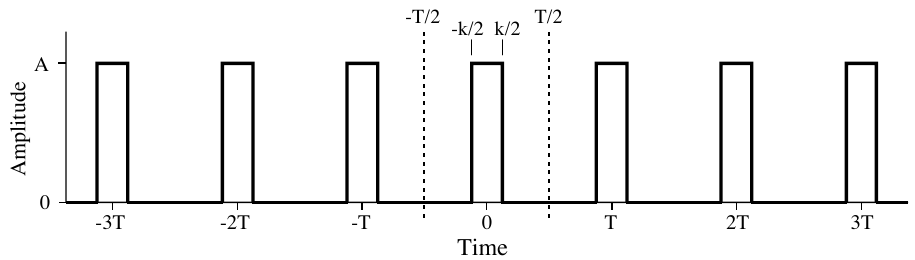
\includegraphics[width=0.762\linewidth,height=0.8\textheight,keepaspectratio]{assets/ch13/fig13-11.png}
\caption*{\textbf{图 13-11　计算傅里叶级数的例子。} 这是一个占空比 d = k/T
的脉冲串。傅里叶级数系数通过在任意一个完整周期上把波形与余弦、正弦波做相关来计算。本例用的是
−T/2 到 T/2 这个周期。 （Amplitude = 幅度，Time = 时间。）}
\end{figure}

于是波形的占空比(duty cycle，脉冲处于''高''电平的时间比例)为 d =
k/T。计算公式 13-5 就能求出傅里叶级数系数。先求直流分量 a₀：

\[
\begin{aligned}
a_0 &= \frac{1}{T}\int_{-T/2}^{T/2} x(t)\, dt && \text{（从公式 13-5 出发）}\\
a_0 &= \frac{1}{T}\int_{-k/2}^{k/2} A\, dt && \text{（代入信号）}\\
a_0 &= \frac{Ak}{T} && \text{（计算积分）}\\
a_0 &= A d && \text{（代入 d = k/T）}
\end{aligned}
\]

这个结果在直觉上说得通：直流分量就是信号的平均值。类似的分析给出''a''系数：

\[
\begin{aligned}
a_n &= \frac{2}{T}\int_{-T/2}^{T/2} x(t)\cos\!\left(\frac{2\pi t n}{T}\right) dt && \text{（从公式 13-5 出发）}\\
a_n &= \frac{2}{T}\int_{-k/2}^{k/2} A\cos\!\left(\frac{2\pi t n}{T}\right) dt && \text{（代入信号）}\\
a_n &= \frac{2A}{T}\,\frac{T}{2\pi n}\left[\sin\!\left(\frac{2\pi t n}{T}\right)\right]_{-k/2}^{k/2} && \text{（计算积分）}\\
a_n &= \frac{2A}{n\pi}\sin(\pi n d) && \text{（化简）}
\end{aligned}
\]

\begin{quote}
\textbf{译注：} 原书这组推导的第一行注明''start with Eq.
13-4''，应为公式 13-5（分析方程），上面已改正。
\end{quote}

``b''系数用同样的方法计算，不过它们全都为零。换句话说，这个波形只用余弦波就能构造出来，不需要正弦波。

如果把时域波形左右平移，``a''和''b''系数会发生变化。例如，本例中的''b''系数只有在某个脉冲以
t = 0 为中心时才为零。可以这样想：如果波形是偶的（即关于 t = 0
对称），它就只由偶的正弦型波（也就是余弦波）组成，于是所有''b''系数都为零。如果波形是奇的（即关于
t = 0
对称但符号相反），它就由奇的正弦型波（即正弦波）组成，于是''a''系数为零。如果把系数换成极坐标形式（比如
M\textsubscript{n} 和 θ\textsubscript{n}
系数），时域的平移不改变幅度，但会给相位加上一个线性分量。

为了把这个例子做完整，设想电子电路中有一个频率为 1
kHz、幅度为一伏、占空比为 0.2 的脉冲串。图 13-12
中的表格给出了这个波形所含各次谐波的幅度。图 13-12
还展示了只用前十四个谐波合成的波形。即使用了这么多谐波，重建效果也不太好。用数学行话说，傅里叶级数收敛得很慢。这只是换一种方式说：时域波形中的陡峭边沿会在频谱中产生非常高的频率。最后，一定要注意陡峭边沿处的过冲，即第
11 章讨论过的吉布斯效应(Gibbs effect)。

\begin{figure}[htbp]
\centering
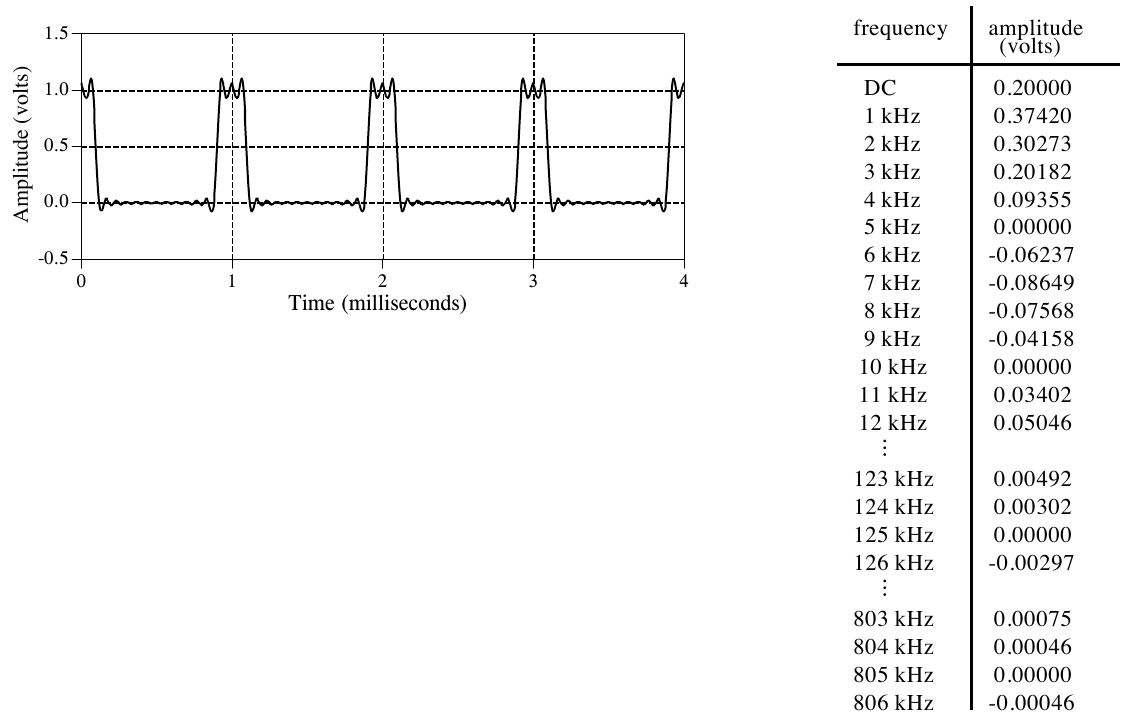
\includegraphics[width=0.942\linewidth,height=0.8\textheight,keepaspectratio]{assets/ch13/fig13-12.png}
\caption*{\textbf{图 13-12　傅里叶级数合成的例子。} 被构造的波形是一个 1
kHz、幅度一伏、占空比 0.2 的脉冲串（如图 13-11
所示）。表格列出了各次谐波的幅度，曲线图则是只用前十四个谐波重建出的波形。
（Amplitude (volts) = 幅度（伏），Time (milliseconds) =
时间（毫秒）；表头 frequency = 频率，amplitude (volts) = 幅度（伏），DC
= 直流。表中数值就是 \(a_n = \frac{2}{n\pi}\sin(0.2\pi n)\)，例如 1
kHz：\(\frac{2}{\pi}\sin(0.2\pi) \approx 0.37420\)；每到 5 的倍数 kHz
恰好为 0。）}
\end{figure}

傅里叶级数的一个重要应用是电子倍频(frequency
multiplication)。假设你要做一个非常稳定的 150 MHz
正弦波振荡器，比如工作在这个频率的无线电发射机可能就需要它。高稳定性要求电路由晶体控制，也就是说，振荡器的频率由电路中一块谐振的石英晶体决定。问题是，石英晶体只能工作到大约
10 MHz。解决办法是先做一个工作在 1～10 MHz
之间某个频率的晶控振荡器，再把频率倍增到所需的值。做法是让正弦波失真，比如用二极管削掉波峰，或者让波形通过一个平方电路。然后用带通滤波器把失真波形中的谐波分离出来。这样频率就能翻两倍、三倍，甚至乘以更高的整数。最常用的技术是用几级二倍频器和三倍频器串起来实现所需的倍频，而不是只用一级。傅里叶级数对这类设计很重要，因为它描述了倍频后信号的幅度，而这个幅度取决于失真的类型和所选的谐波。
